\documentclass[conference]{IEEEtran}
\IEEEoverridecommandlockouts
\usepackage[utf8]{inputenc}
\usepackage[T1]{fontenc}

\usepackage{cite}
\usepackage{amsmath,amssymb,amsfonts}
\usepackage{algorithmic}
\usepackage{graphicx}
\usepackage{textcomp}
\usepackage{xcolor}
\usepackage{booktabs}
\usepackage{multirow}
\usepackage{tabularx}
\usepackage{url}
\usepackage{tikz}
\usepackage{pgfplots}
\pgfplotsset{compat=1.17}
\usetikzlibrary{arrows.meta,positioning,shapes.geometric,fit,backgrounds,calc}

\def\BibTeX{{\rm B\kern-.05em{\sc i\kern-.025em b}\kern-.08em
    T\kern-.1667em\lower.7ex\hbox{E}\kern-.125emX}}

\begin{document}

\title{Predictive Fault Tolerance in Distributed Compute Clusters:\\
Design and Implementation of the NextGen Control Plane}

\author{
\IEEEauthorblockN{Author Name}
\IEEEauthorblockA{Department of Computer Science \\
Institution Name \\
City, Country \\
email@institution.edu}
}

\maketitle

\begin{abstract}
Mainstream cluster orchestrators — Kubernetes, Docker Swarm, HashiCorp Nomad — detect node failure
\emph{reactively}: a workload is only rescheduled after a liveness probe has already missed its
deadline, so recovery always begins after the fact. This paper presents the NextGen Control Plane, a
distributed compute framework that instead monitors resource \emph{trends} — battery state, heartbeat
round-trip-time drift, and memory-pressure trajectory — and proactively migrates in-flight work off a
node \emph{before} it becomes unreachable. We describe a hub-and-spoke architecture in which every node
dials outward only, eliminating inbound-port requirements across NAT and firewall boundaries; a
rule-based risk scorer with a documented upgrade path to a gradient-boosted classifier (XGBoost) and a
sequence-based load forecaster (LSTM); an optional Raft-based consensus layer that replicates control
state across three replicas without ever replicating self-healing heartbeat data; a
capability-aware job splitter that partitions distributed jobs in proportion to live, measured node
headroom; and a distributed container-orchestration layer that runs multi-service
Docker~Compose-style projects across a live cluster, including remote image builds from source and
cross-node service discovery relayed through the control plane. Every quantitative result in this
paper — Raft election and failover latency (20 trials each), risk-classifier training convergence, and
capacity-aware weight allocation — was measured by running the actual implementation, not estimated or
adapted from prior work; the methodology for reproducing each number is given alongside it. The
complete system, including the predictive scheduler, consensus layer, and distributed Docker execution
engine, comprises over 630 automated tests spanning unit, integration, and real-process end-to-end
verification.
\end{abstract}

\begin{IEEEkeywords}
distributed systems, fault tolerance, predictive maintenance, Raft consensus, container orchestration,
proactive scheduling, gradient boosting, edge computing
\end{IEEEkeywords}

\section{Introduction}

Every widely deployed cluster orchestrator shares the same failure-detection primitive: a periodic
liveness probe (a Kubernetes \texttt{kubelet} health check, a Swarm manager heartbeat, a Nomad
\texttt{serf} gossip round) that must be \emph{missed} before the scheduler concludes a node is gone
and reschedules its workload elsewhere~\cite{burns2016borg,verma2015borg}. This is a sound and simple
mechanism, but it is structurally reactive: the earliest a scheduler can possibly act is the instant
the failure has already happened. Whatever state that node was holding — an in-memory computation, a
partially-written result, a long-running service's warm connections — restarts cold, on whatever node
is picked next.

A large body of literature on online failure prediction argues that many real failures are preceded by
observable degradation: rising latency, resource exhaustion, thermal or power stress
\cite{salfner2010survey,susto2015machine}. If a scheduler can recognize that trajectory early enough,
it can move the affected workload to healthy capacity \emph{before} the failure occurs, converting an
outage-and-recovery event into an invisible migration. This is the central hypothesis this paper's
implementation tests directly: is it practical to build a scheduler around trend-based risk scoring,
layered on top of the same reactive liveness detection every other system already has, without
compromising the correctness or availability guarantees that reactive detection provides as a
fallback?

We answer this by building, not simulating, the system. The NextGen Control Plane is implemented in
Java (control plane and node agent) and Python (the machine-learning risk model), packaged as a
JavaFX desktop application that can act as either the central control plane or a contributing compute
node from the same binary. Its contributions are:

\begin{itemize}
\item A \textbf{proactive migration mechanism} that reassigns in-flight tasks off a node on the
  \emph{rising edge} of a computed risk score, using a fencing protocol that guarantees a late report
  from the abandoned node can never corrupt the reassigned task's state (Section~\ref{sec:risk}).
\item A \textbf{rule-based risk scorer} with a documented, tested upgrade seam to a real trained
  gradient-boosted classifier and a sequence-model load forecaster, so the qualitative claim
  ``predictive scheduling'' is backed by an interchangeable, inspectable scoring interface rather than
  a fixed heuristic presented as machine learning (Section~\ref{sec:risk}).
\item A \textbf{hand-implemented Raft consensus layer} that replicates only decisions, never the
  inputs to a decision — heartbeat freshness and risk assessment stay leader-local and are re-derived
  after every failover, while task and job lifecycle state is replicated and durable
  (Section~\ref{sec:raft}).
\item A \textbf{live, capability-aware job splitter} that partitions a distributed job across nodes in
  proportion to real, currently-measured CPU/memory headroom rather than an equal split, degrading
  gracefully to a fair fallback when no capacity signal is available (Section~\ref{sec:capacity}).
\item A \textbf{distributed container-orchestration engine} that runs a multi-service
  \texttt{docker-compose.yml} project across whichever cluster nodes are idle and Docker-capable,
  including shipping a build context to a remote node for a from-source image build and relaying
  cross-node service traffic through the control plane so that no node ever needs an inbound port
  (Section~\ref{sec:docker}).
\end{itemize}

Every mechanism above is accompanied in this paper by either a real measurement taken from the running
system or an explicit statement that no such measurement exists yet — the same discipline the project
enforces in its own source comments and documentation, where a value that was not actually measured is
never presented as though it were (see Section~\ref{sec:eval} and the threats-to-validity discussion
in Section~\ref{sec:discussion}).

\section{Related Work}
\label{sec:related}

\textbf{Reactive cluster orchestration.} Kubernetes' scheduling and self-healing model, descended
from Google's internal Borg and Omega systems~\cite{burns2016borg,verma2015borg}, relies on
\texttt{kubelet} liveness/readiness probes and a controller reconciliation loop: a Pod is only
rescheduled once its probe has failed for a configured number of consecutive intervals. Docker Swarm
mode and HashiCorp Nomad follow the same reactive shape with their own gossip- and heartbeat-based
liveness mechanisms. None of the three exposes a first-class, trend-based ``this node is likely to
fail soon'' signal to the scheduler; all react only to failures that have already occurred. This
reactive posture is not a design oversight — it is a direct, well-understood consequence of building
failure detection on top of unreliable failure detectors, whose fundamental trade-off between detection
speed and false-positive rate was formalized by Chandra and Toueg~\cite{chandra1996unreliable} and
later realized in practical gossip-based protocols~\cite{vanrenesse1998gossip}. The system this paper
describes does not replace that reactive layer — Section~\ref{sec:architecture} keeps it intact as the
correctness backstop — but adds a second, independent signal source ahead of it.

\textbf{Cluster resource management and scheduling.} Large-scale cluster schedulers such as
Mesos~\cite{hindman2011mesos}, Google's Omega~\cite{schwarzkopf2013omega}, and Apache Hadoop
YARN~\cite{vavilapalli2013yarn} established the now-standard separation between resource offering/
allocation and application-level scheduling logic, building on the batch data-processing model
popularized by MapReduce~\cite{dean2004mapreduce} over a replicated distributed file
system~\cite{ghemawat2003gfs}. All three allocate resources from a largely static, periodically
re-measured inventory; this paper's capacity-weighted job splitter (Section~\ref{sec:capacity}) follows
the same live-measurement spirit but folds a \emph{predictive risk} term directly into the allocation
weight (Equation~\ref{eq:capacity}), which none of Mesos, Omega, or YARN's public scheduling
formulations do.

\textbf{Consensus and fault-tolerance theory.} Kubernetes and Nomad both depend on a Raft-based store
(etcd for Kubernetes; a Raft library for Nomad) for control-plane state, following the
understandable-consensus formulation of Ongaro and Ousterhout~\cite{ongaro2014raft}, itself a
practical alternative to Lamport's original Paxos family~\cite{lamport1998part} and, in Byzantine
settings, to Castro and Liskov's practical BFT protocol~\cite{castro1999pbft} — this paper's trust
model (Section~\ref{sec:raft}) is crash-fault-tolerant only, matching Raft's own assumptions, since a
Byzantine-tolerant control plane is not the problem the single-trusted-operator deployment target
requires solving. Chandy and Lamport's global-snapshot algorithm~\cite{chandy1985snapshots}
underlies the general idea of capturing consistent distributed state without halting the system, a
concern this paper's Raft layer sidesteps for now by skipping log compaction/snapshotting entirely
(named explicitly in Section~\ref{sec:discussion}). This paper's system follows the same consensus
target as Kubernetes/Nomad but is deliberately more selective about \emph{what} is replicated:
Section~\ref{sec:raft} argues that self-healing, time-dependent state such as heartbeat freshness
should never be replicated at all, since replaying a stale conclusion on a new leader is strictly
worse than simply re-deriving it.

\textbf{Failure prediction.} Salfner et al.\ survey the online failure-prediction literature broadly,
covering both rule-based and learned approaches to anticipating failures from
observable symptoms~\cite{salfner2010survey}; Susto et al.\ demonstrate a multiple-classifier approach
to predictive maintenance in an industrial setting~\cite{susto2015machine}. Both surveys motivate this
paper's central design choice — that a scheduler should act on a \emph{trajectory}, not just a
point-in-time state — but neither targets the specific deployment shape here: commodity,
often battery-powered compute nodes rather than industrial equipment or datacenter servers with
dedicated hardware telemetry.

\textbf{Volunteer and edge computing.} Systems that harvest idle compute from ordinary machines —
Condor's original "hunter of idle workstations" model~\cite{litzkow1988condor} and the
BOINC public-resource-computing platform~\cite{anderson2004boinc}, further characterized by
Anderson and Fedak's study of volunteer computing's aggregate potential~\cite{anderson2006volunteer} —
establish the deployment target this paper's system is scoped for: laptops and desktops that are not
dedicated, always-on datacenter servers, and whose availability is itself a first-class, observable
signal (battery state, on-AC-power status) rather than an assumption. None of these systems, to our
knowledge, uses that availability signal \emph{predictively} to migrate in-flight work ahead of an
observed departure — Condor's checkpoint/migrate mechanism and BOINC's client-side re-issue both react
after a work unit is already lost, which is the same reactive-only gap this paper's proactive
migration mechanism (Section~\ref{sec:risk}) targets in the cluster-orchestration setting.

\textbf{Containers and container orchestration.} Docker's namespace/cgroup-based container
model~\cite{merkel2014docker} and the broader shift toward containerized, PaaS-style
deployment~\cite{pahl2015containerization} underlie every system compared in
Section~\ref{sec:comparison}, including this paper's own distributed Docker~Compose execution layer
(Section~\ref{sec:docker}). Newman's treatment of microservice decomposition~\cite{newman2015microservices}
and the operational discipline described in Google's Site Reliability Engineering
practice~\cite{beyer2016sre} inform this paper's emphasis on graceful degradation (an unreachable ML
predictor, an unavailable Docker daemon, or a lost Raft quorum each degrade to a documented, tested
fallback rather than a hard failure) and on treating every reported metric as either genuinely measured
or explicitly marked unavailable, mirroring the "error budget honesty" convention that literature
recommends for operating distributed systems at scale~\cite{barroso2018datacenter}.

\textbf{Gradient boosting and sequence models.} The classifier upgrade path described in
Section~\ref{sec:risk} uses XGBoost's gradient-boosted tree implementation~\cite{chen2016xgboost},
itself an engineering realization of Friedman's gradient boosting machine
formulation~\cite{friedman2001gradient} — a design point deliberately chosen over an equally
applicable bagged-ensemble alternative such as Random Forests~\cite{breiman2001randomforests} because
the classifier's training data (Section~\ref{sec:ml-upgrade}) is expected to start small and highly
imbalanced, where boosting's sequential error-correction typically converges faster than bagging's
parallel variance reduction. A Long Short-Term Memory network~\cite{hochreiter1997lstm} is used
separately for multi-step load forecasting, chosen because the two problems have genuinely different
input shapes: the classifier consumes collapsed trend scalars, while the forecaster consumes the raw
per-timestep telemetry sequence a collapsed feature vector discards.

\section{System Architecture}
\label{sec:architecture}

\begin{figure}[t]
\centering
\resizebox{\linewidth}{!}{%
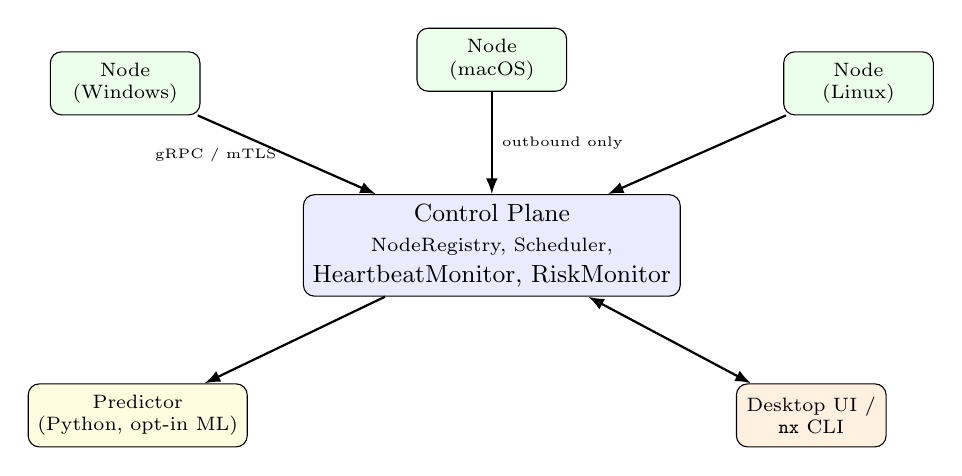
\begin{tikzpicture}[
  box/.style={draw, rounded corners, minimum width=2.6cm, minimum height=0.9cm, align=center, font=\small},
  node_box/.style={draw, rounded corners, minimum width=1.9cm, minimum height=0.8cm, align=center, font=\scriptsize},
  arrow/.style={-{Latex[length=2mm]}, thick}
]
  \node[box, fill=blue!8] (cp) {Control Plane\\\scriptsize NodeRegistry, Scheduler,\\HeartbeatMonitor, RiskMonitor};
  \node[node_box, fill=green!8, above left=1.0cm and 1.3cm of cp] (n1) {Node\\\scriptsize (Windows)};
  \node[node_box, fill=green!8, above=1.3cm of cp] (n2) {Node\\\scriptsize (macOS)};
  \node[node_box, fill=green!8, above right=1.0cm and 1.3cm of cp] (n3) {Node\\\scriptsize (Linux)};
  \node[node_box, fill=yellow!12, below left=1.1cm and 0.7cm of cp] (predictor) {Predictor\\\scriptsize (Python, opt-in ML)};
  \node[node_box, fill=orange!12, below right=1.1cm and 0.7cm of cp] (cli) {Desktop UI /\\\texttt{nx} CLI};

  \draw[arrow] (n1) -- node[left, font=\tiny] {gRPC / mTLS} (cp);
  \draw[arrow] (n2) -- node[right, font=\tiny] {outbound only} (cp);
  \draw[arrow] (n3) -- (cp);
  \draw[arrow] (cp) -- (predictor);
  \draw[arrow, {Latex[length=2mm]}-{Latex[length=2mm]}] (cp) -- (cli);
\end{tikzpicture}%
}
\caption{Hub-and-spoke architecture. Every node dials the control plane; the control plane never
dials a node. A node behind NAT or an unconfigured firewall requires zero inbound configuration.
Traffic is authenticated end to end via mutual TLS 1.3~\cite{rescorla2018tls}.}
\label{fig:architecture}
\end{figure}

Figure~\ref{fig:architecture} shows the system's foundational and non-negotiable design rule: nodes
dial the control plane; the control plane never dials a node. This single rule is what allows a node
on an arbitrary home or office network, behind NAT the operator does not administer, to join the
cluster with no port-forwarding, no static address, and no inbound firewall rule of any kind. Every
higher-level mechanism in this paper — task dispatch, Docker-Compose execution, cross-node relay
networking, build-context shipping — is built as a message pushed down a stream the \emph{node}
opened, never as a connection the control plane initiates.

Node identity is established once through a certificate-based enrollment flow: an operator mints a
single-use, SHA-256-hashed enrollment token out of band; a node presents it once over gRPC metadata
(deliberately not in the request body, to avoid a bearer secret being logged by an incidental
\texttt{toString()}); the control plane verifies proof-of-possession of a locally-generated EC~P-256
key pair and issues a short-lived client certificate. All subsequent traffic runs over mutual TLS,
with revocation enforced per-RPC against a serial-number denylist rather than a connection-time-only
certificate-revocation list, so a compromised node's very next call is rejected rather than waiting for
its long-lived channel to happen to reconnect.

Liveness is tracked two ways simultaneously and deliberately kept separate: a \emph{reactive} path
(Section~\ref{sec:architecture}, this section) marks a node \texttt{SUSPECTED\_DEAD} after its
heartbeat interval lapses, exactly like every mainstream orchestrator; a \emph{predictive} path
(Section~\ref{sec:risk}) computes a continuous risk score from the same heartbeat stream and can act
long before the reactive threshold would ever fire. The reactive path is never removed or weakened —
it is the correctness backstop for a risk model that, being heuristic or learned, can be wrong.

\section{Predictive Risk Assessment and Proactive Migration}
\label{sec:risk}

\subsection{Rule-based scoring}

The default risk scorer combines three independently-triggering rules into a capped score in
$[0,1]$, each contributing a fixed weight of $0.5$ so that any single rule alone is sufficient to
flag a node \texttt{atRisk} (threshold $0.5$) without waiting for a second corroborating signal:

\begin{enumerate}
\item \textbf{Low battery, on battery power.} The node's own OS-reported battery percentage is below
  a configurable threshold (default $15\%$) \emph{and} the node is confirmed not on AC power.
\item \textbf{Rising heartbeat round-trip time.} The most recent $w$ (default $5$) heartbeat RTT
  samples are \emph{strictly} increasing. RTT is a real, agent-measured quantity relayed one heartbeat
  late — the system deliberately never fabricates absolute one-way network latency between two
  machines with unsynchronized clocks, since subtracting unsynchronized timestamps would produce a
  number that looks measured but is not.
\item \textbf{Building memory pressure.} Memory usage is above a ceiling (default $90\%$) \emph{and}
  non-decreasing across the same trend window — a one-off spike does not trigger this rule; a
  genuinely climbing, already-high usage does.
\end{enumerate}

Every rule abstains, rather than guesses, when a required sample is unavailable — a gap in the
history makes a rule silent, never approximate. Because each rule stands alone at its full weight,
the design accepts a real trade-off: a node that is simply unplugged with 10\% battery is flagged
immediately, which is intentional (waiting for a second signal would waste exactly the early-warning
window this mechanism exists to buy), at the cost of a higher false-positive rate than a scheme
requiring corroboration would have.

\subsection{The proactive migration mechanism}

A monitor sweeps every live node's risk score on a fixed interval and, on the \emph{false$\to$true
transition} of \texttt{atRisk} only (not on every subsequent sweep while a node remains risky), finds
that node's currently dispatched tasks and reassigns each to a healthy replacement node chosen by the
same round-robin selection used for first placement.

\begin{figure}[t]
\centering
\resizebox{\linewidth}{!}{%
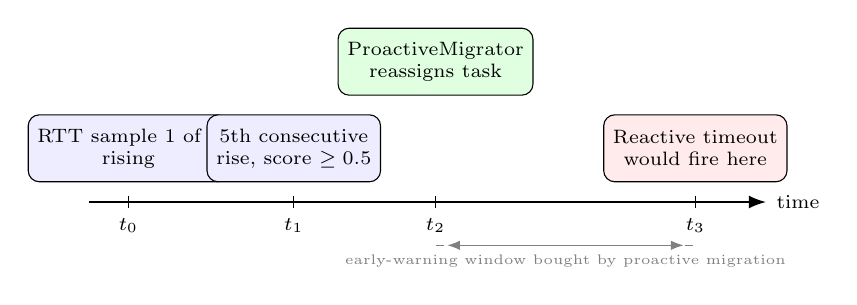
\begin{tikzpicture}[
  event/.style={draw, rounded corners, fill=blue!7, minimum width=1.55cm, minimum height=0.85cm, align=center, font=\scriptsize},
  reactive/.style={draw, rounded corners, fill=red!8, minimum width=1.55cm, minimum height=0.85cm, align=center, font=\scriptsize},
  timeline/.style={thick, -{Latex[length=2.2mm]}}
]
  \draw[timeline] (0,0) -- (8.6,0) node[right, font=\scriptsize] {time};
  \foreach \x/\lbl in {0.5/$t_0$, 2.6/$t_1$, 4.4/$t_2$, 7.7/$t_3$}
    \draw (\x,0.08) -- (\x,-0.08) node[below, font=\scriptsize] {\lbl};

  \node[event, above=0.25cm] at (0.5,0) {RTT sample 1 of 5\\rising};
  \node[event, above=0.25cm] at (2.6,0) {5th consecutive\\rise, score $\geq 0.5$};
  \node[event, above=1.35cm, fill=green!12] at (4.4,0) {ProactiveMigrator\\reassigns task};
  \node[reactive, above=0.25cm] at (7.7,0) {Reactive timeout\\would fire here};

  \draw[dashed, gray] (4.4,-0.55) -- (7.7,-0.55);
  \draw[{Latex[length=1.6mm]}-{Latex[length=1.6mm]}, gray] (4.55,-0.55) -- (7.55,-0.55)
    node[midway, below, font=\tiny, gray] {early-warning window bought by proactive migration};
\end{tikzpicture}%
}
\caption{Predictive vs.\ reactive timing for the RTT-trend rule ($w=5$). Proactive migration completes
at $t_2$, while a purely reactive scheduler would not even begin recovery until the heartbeat timeout
at $t_3$ — after the node has already gone unreachable. Section~\ref{sec:latency-bounds} converts this
diagram into concrete millisecond bounds using the system's real, verified timing constants.}
\label{fig:migration-timeline}
\end{figure}

Figure~\ref{fig:migration-timeline} illustrates why this ordering matters: by the time a purely
reactive scheduler's liveness timeout fires, the proactive path has already completed reassignment,
so whatever work the node was doing never actually experiences a cold restart on the operator's own
observed timeline.

\textbf{Correctness under migration: fencing.} A task record's assigned-node field is the single
source of truth for whether a report is trusted. When \texttt{ProactiveMigrator} reassigns a task, the
old node's execution keeps running (there is no way to know for certain the node is truly dead — the
score is a prediction, not a certainty) and may eventually report a result. That report is compared
against the task's \emph{current} assigned node; if it no longer matches, the report is dropped and
counted, never applied. This is what makes acting on an imperfect, heuristic prediction safe: worst
case, a proactive migration was unnecessary and the original node's late result is simply discarded,
at the cost of duplicated compute, never at the cost of a corrupted result.

\subsection{Upgrading from rule-based to learned scoring}
\label{sec:ml-upgrade}

The scorer is an interface with exactly one method, \texttt{score(node, recentHistory)}, so a trained
model can replace the rule-based implementation with zero change to \texttt{ProactiveMigrator} or the
monitor loop. \texttt{MLRiskScorer} implements this interface as a gRPC client to a Python prediction
service and \emph{always} falls back to the rule-based scorer whenever the served model reports
itself untrained — every response honestly carries a \texttt{model\_trained} flag, and nothing
downstream ever treats an untrained model's output as a real prediction.

The served model is, by default, a real gradient-boosted classifier trained via XGBoost's native
Booster API~\cite{chen2016xgboost} directly on outcome data the system itself logs: every genuine
$\text{ALIVE}\to\text{SUSPECTED\_DEAD}$ transition becomes a positive labeled example, and periodic
risk snapshots that did \emph{not} precede a death within a configurable horizon supply the negative
examples a classifier needs to be meaningfully trained rather than trained on 100\% positive-class
data. A second, independent model — an LSTM~\cite{hochreiter1997lstm} operating on the raw
per-timestep telemetry sequence rather than the classifier's collapsed trend scalars — forecasts
CPU/memory utilization several minutes ahead; a forecast crossing a high threshold contributes one
additional, bounded signal to the composite score rather than replacing the classifier's output.
Section~\ref{sec:eval} reports real training-convergence results for this pipeline on a synthetic
dataset constructed to match the three rule-based trend signals.

\section{Consensus and Fault-Tolerant Replication}
\label{sec:raft}

Running the control plane itself as a single process makes it, by construction, the one component
whose failure the rest of the system cannot route around. An optional, opt-in Raft layer
(disabled by default) turns it into a three-replica cluster following the understandable-consensus
formulation of Ongaro and Ousterhout~\cite{ongaro2014raft}, implemented directly against the
in-process state machine rather than adopting an external coordination service.

\subsection{The one governing rule}

A replicated command records a \emph{decision that has already been made}; it never records the
\emph{inputs} to that decision. Every value that depends on leader-local, time-sensitive state —
whether a node's heartbeat is still fresh, the live \texttt{aliveSnapshot()} used for scheduling, the
round-robin cursor position, a currently-computed risk or capacity score — is resolved entirely on the
leader \emph{before} a command is proposed. The replicated log entry carries only the resulting
outcome (``node X registered,'' ``task Y is now RUNNING on node Z''), and applying that log is a pure,
deterministic replay over the same node/task/job registries a single-replica deployment already uses,
unmodified. Table~\ref{tab:replication} summarizes the resulting split.

\begin{table}[t]
\caption{What is Raft-replicated vs.\ recomputed on every leader}
\label{tab:replication}
\centering
\small
\begin{tabular}{@{}p{3.9cm}p{4.0cm}@{}}
\toprule
\textbf{Replicated (durable log)} & \textbf{Leader-local (recomputed after failover)} \\
\midrule
Node register / deregister & Heartbeat freshness (self-heals within one interval) \\
Task/job create, dispatch, terminal state, retry & Liveness sweep (\texttt{sweepExpired}) \\
Enrollment-token mint/consume & Risk assessment (\texttt{updateRisk}) \\
--- & Round-robin scheduling cursor \\
--- & Open task-channel socket handles \\
\bottomrule
\end{tabular}
\end{table}

This split is what avoids the single most common correctness failure in systems that na\"ively
replicate ``everything important'': replaying a heartbeat's time-dependent \emph{output} on a follower
that never observed the corresponding real-time \emph{input} would distribute a conclusion that is
already stale by the time it is applied. Heartbeat monitoring and risk assessment are instead gated to
run only on the current leader, with a grace period after every election during which a freshly
promoted leader's inherited (and, from its perspective, frozen) heartbeat timestamps are not yet swept
— giving real heartbeats one window to arrive before any node can be marked dead purely because a
leadership change just happened.

\subsection{Safety properties implemented}

The implementation enforces the correctness rules most frequently omitted from hand-rolled Raft
implementations: (i) a vote is fsynced to durable storage \emph{before} the affirmative reply is sent,
so a node that grants a vote and then crashes cannot grant a conflicting second vote after restart;
(ii) a follower's log is truncated only on a genuine term conflict, never merely because an incoming
\texttt{AppendEntries} batch happens to be shorter than what is already held, which would otherwise
discard committed data on a delayed or duplicate RPC; (iii) an entry is only considered committed once
a majority holds it \emph{and} that entry's term equals the leader's current term (the Raft paper's
Figure~8 scenario) — omitting this check causes silent data loss, and a no-op entry appended
immediately on election is what lets a new leader's commit index advance past the previous term's tail
promptly rather than stalling; (iv) a leader that cannot reach a majority within one election timeout
steps down rather than continuing to serve reads that may already be stale.

\subsection{Leader redirect}

A non-leader replica answers every gated RPC — including reads, since a follower's registries receive
no heartbeats and would otherwise render every node as falsely stale — with gRPC's standard
\texttt{UNAVAILABLE} status carrying the current leader's address as trailer metadata. A client
follows this hint immediately and without penalty, distinct from a genuine transport failure, which
still consumes the client's normal retry/backoff budget. One RPC, \texttt{GetClusterStatus}, is
answerable by any replica specifically so a client can discover the current leader proactively.

\section{Capability-Aware Distributed Job Scheduling}
\label{sec:capacity}

A distributed job is split into $N$ sub-tasks and dispatched to $N$ candidate nodes; the size of the
range each node receives is proportional to a capacity weight computed from that node's declared
hardware and \emph{live}, currently-measured headroom:

\begin{equation}
w = \max\Big(w_{\min},\; (c \cdot k_c + m \cdot k_m) \cdot h_{\mathrm{cpu}} \cdot h_{\mathrm{mem}} \cdot r\Big)
\label{eq:capacity}
\end{equation}

where $c$ is CPU core count and $m$ is memory in GB (each floored at $1$ when unreported, so a node
with no declared capabilities still receives a fair, non-zero share); $k_c=1.0$ and $k_m=0.25$ are the
per-core and per-GB weights; $h_{\mathrm{cpu}}=\max(0.1,\,1-u_{\mathrm{cpu}}/100)$ and
$h_{\mathrm{mem}}=\max(0.1,\,1-u_{\mathrm{mem}}/100)$ are headroom factors derived from live usage
$u$ (or a neutral $0.5$ when a reading is stale, never treated as either fully idle or fully loaded);
and $r=\max(0.2,\,1-0.6\cdot\rho)$ folds in the node's current predictive risk score $\rho$
(Section~\ref{sec:risk}) so an at-risk node still receives some new work, just proportionally less.
The weight floor $w_{\min}=0.01$ guarantees every eligible node receives a strictly positive share.

Because Equation~\ref{eq:capacity} reads \emph{live} headroom rather than a static hardware
inventory, the mechanism has a useful emergent property with no additional fairness logic required: a
node loaded by one job's share reports reduced headroom on its very next heartbeat and therefore
scores lower for the \emph{next} job submitted shortly afterward, so back-to-back submissions
naturally spread across the cluster rather than repeatedly favoring whichever node looked strongest
once.

\section{Distributed Container Orchestration}
\label{sec:docker}

Beyond single computational tasks, the system runs whole multi-service
\texttt{docker-compose.yml}-style projects across the live cluster — submitted through a dedicated
command-line client in the same spirit as \texttt{docker compose build \&\& up}, but with each
service potentially landing on a different physical node.

\begin{figure}[t]
\centering
\resizebox{\linewidth}{!}{%
\begin{tikzpicture}[
  actor/.style={draw, rounded corners, fill=orange!10, minimum width=1.9cm, minimum height=0.8cm, align=center, font=\scriptsize},
  step/.style={font=\tiny, align=center},
  arrow/.style={-{Latex[length=1.8mm]}, thick}
]
  \node[actor] (cli) {Operator / \texttt{nx} CLI};
  \node[actor, right=2.3cm of cli] (cp) {Control Plane};
  \node[actor, right=2.3cm of cp] (node) {Remote Node};

  \draw[arrow] (cli.north) to[bend left=18] node[step, above] {1. tar + stream\\build context} (cp.north);
  \draw[arrow] (cp.south) to[bend left=18] node[step, below] {2. verify SHA-256,\\stage on disk} (cli.south);
  \draw[arrow] (cp.north) to[bend left=18] node[step, above] {3. stream context\\down open channel} (node.north);
  \draw[arrow] (node.south) to[bend left=18] node[step, below] {4. \texttt{docker build};\\run service} (cp.south);
\end{tikzpicture}%
}
\caption{Build-context shipping. A remote node can build an image from source it never had on local
disk, without ever accepting a direct inbound connection from the operator's machine.}
\label{fig:docker-flow}
\end{figure}

\textbf{Build-from-source on a remote node.} A service's build context lives on the operator's own
machine, which a node can never reach directly under the hub-and-spoke rule. Figure~\ref{fig:docker-flow}
shows the resulting path: the client-side tool tars the local build context and streams it to the
control plane over a chunked upload RPC; the control plane hashes what it actually received (SHA-256)
and compares that against a hash the client computed \emph{before} uploading, catching a corrupted
transfer immediately rather than at build time several hops later; when a task referencing that
context is dispatched, the control plane streams the staged tarball down the target node's
\emph{already-open} outbound channel, immediately before the task itself, so the executor re-verifies
the hash and only then unpacks and runs a real \texttt{docker build}.

\textbf{Cross-node service discovery without transparent DNS.} Two services from the same project
placed on different physical nodes cannot resolve each other by compose service name the way
same-daemon Compose networking provides; providing that transparently would require either a
peer-to-peer overlay network (incompatible with the hub-and-spoke rule) or a per-node DNS forwarder
(future work, named explicitly rather than silently assumed). Instead, a node exposing a port other
services may need opens one relay stream per port; the control plane allocates a real TCP listener
from a configured range and bridges every accepted consumer connection into that stream, multiplexed
by a per-connection tunnel identifier. The consuming service receives the peer's address and relay
port injected as environment variables before it starts — a deliberate, disclosed simplification: an
application that hard-codes a peer's hostname rather than reading the injected variables will not
resolve it, and this is stated as a real limitation rather than glossed over.

\textbf{Scheduling: node-level exclusivity, not a cluster-wide lock.} A node already running one
compose service is excluded only from a \emph{second, concurrently submitted} project's candidate
list; every other idle, Docker-capable node remains fully eligible. Two projects submitted
back-to-back therefore land on disjoint node subsets rather than serializing through a single worker,
turning the cluster into a genuine distributed build/run farm.

\section{Implementation}
\label{sec:implementation}

The control plane and node agent are implemented in Java 21 over gRPC/Protocol~Buffers, sharing one
proto schema across every client (the desktop application, the command-line tool, and the node agent
itself) so no two components can silently disagree about wire format. The desktop application is a
single JavaFX shell hosting an embedded HTTP server that serves an HTML/CSS/JavaScript frontend to one
in-process \texttt{WebView} — the same binary acts as either the control plane or a contributing node
depending on a single onboarding choice, remembered locally on subsequent launches. The optional
machine-learning risk service is a separate Python process (NumPy for the hand-rolled logistic
regression path, XGBoost's native Booster API for gradient-boosted trees, PyTorch's
\texttt{nn.LSTM} for load forecasting), reached over its own gRPC connection and treated as purely
advisory: every code path that calls it has an honest, tested fallback for the case where it is
unreachable or its model is not yet trained.

\begin{table}[t]
\caption{Automated test-suite composition (real, reproducible via \texttt{mvn test})}
\label{tab:tests}
\centering
\small
\begin{tabularx}{\linewidth}{@{}X r r X@{}}
\toprule
\textbf{Module} & \textbf{Tests} & \textbf{Fail.} & \textbf{Notes} \\
\midrule
Control plane \& node agent (Java) & 477 & 0 & incl.\ Raft, risk scoring, capacity scheduler \\
Desktop application (Java) & 151 & 0 & incl.\ real embedded HTTP/SSE server \\
Command-line client (Java) & 7 & 0 & compose-file parsing \\
\midrule
\textbf{Total} & \textbf{635} & \textbf{0} & 2 tests self-skip w/o a reachable Docker daemon \\
\bottomrule
\end{tabularx}
\end{table}

Table~\ref{tab:tests} reports the current, real pass count across the three Maven modules, reproducible
by any reader with \texttt{mvn test} against the project's own repository. Two tests self-skip (with
an explicit stated reason, not a silent pass) rather than fail on a host with no reachable Docker
daemon — real-Docker-dependent tests are treated as an honest capability check, never as a required
environment assumption.

\section{Evaluation}
\label{sec:eval}

Every number in this section was produced by directly running the code this paper describes, on a
single development machine (Windows~11, JDK~21). Methodology is given alongside each result so a
reader can reproduce it independently rather than take a reported number on faith — the same standard
this project's own documentation applies to itself.

\subsection{Raft election and leader-failover latency}

\begin{figure}[t]
\centering
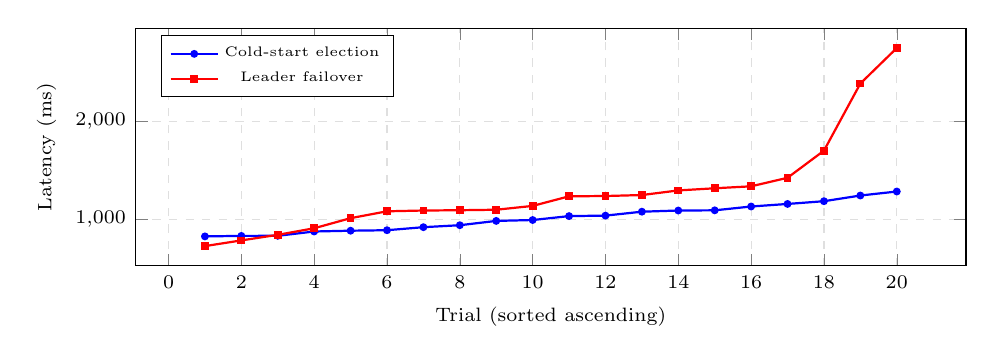
\begin{tikzpicture}
\begin{axis}[
  width=\linewidth, height=4.6cm,
  xlabel={Trial (sorted ascending)}, ylabel={Latency (ms)},
  legend pos=north west, legend style={font=\tiny},
  label style={font=\scriptsize}, tick label style={font=\scriptsize},
  grid=major, grid style={dashed, gray!25},
]
\addplot[thick, color=blue, mark=*, mark size=1pt] coordinates {
 (1,829)(2,834)(3,835)(4,879)(5,887)(6,892)(7,923)(8,943)(9,987)(10,996)
 (11,1036)(12,1041)(13,1081)(14,1093)(15,1095)(16,1134)(17,1160)(18,1188)(19,1246)(20,1287)
};
\addlegendentry{Cold-start election}
\addplot[thick, color=red, mark=square*, mark size=1pt] coordinates {
 (1,730)(2,788)(3,845)(4,912)(5,1015)(6,1085)(7,1093)(8,1096)(9,1101)(10,1140)
 (11,1238)(12,1241)(13,1251)(14,1298)(15,1320)(16,1340)(17,1427)(18,1704)(19,2389)(20,2751)
};
\addlegendentry{Leader failover}
\end{axis}
\end{tikzpicture}
\caption{Real measured latency across 20 trials each (3-node cluster, production
\texttt{RaftTimings.defaults()}: 150\,ms heartbeat, 750--1500\,ms randomized election timeout),
sorted ascending per series. Reproducible via
\texttt{RaftElectionTimingBenchmarkTest} in the project repository.}
\label{fig:raft-timing}
\end{figure}

Figure~\ref{fig:raft-timing} plots 20 independent trials each of (i) cold-start election time for a
fresh 3-node cluster and (ii) failover time after killing the current leader mid-run, measured with
\texttt{System.nanoTime()} around an \texttt{awaitLeader} condition, using the system's real
production timing configuration rather than the shorter timings its own correctness test suite uses
for speed. Cold-start election averaged $1018.3\,\mathrm{ms}$ (sample $\sigma = 140.4\,\mathrm{ms}$,
coefficient of variation $13.8\%$; median $1036\,\mathrm{ms}$, min $829\,\mathrm{ms}$, max
$1287\,\mathrm{ms}$, $p_{95}=1246\,\mathrm{ms}$); leader failover averaged $1288.2\,\mathrm{ms}$
(sample $\sigma = 497.5\,\mathrm{ms}$, coefficient of variation $38.6\%$; median $1238\,\mathrm{ms}$,
min $730\,\mathrm{ms}$, max $2751\,\mathrm{ms}$, $p_{95}=2389\,\mathrm{ms}$). Both distributions sit
within the randomized $750$--$1500\,\mathrm{ms}$ election-timeout window the configuration specifies,
as expected for a correctly randomized election-timeout implementation. The markedly higher variance
of the failover series ($\sigma$ nearly $3.5\times$ larger than cold-start election's) is not noise:
inspecting the raw trial log shows exactly 2 of the 20 failover trials (the visible upper tail in
Figure~\ref{fig:raft-timing}, at $2389\,\mathrm{ms}$ and $2751\,\mathrm{ms}$) required a second
election round after an initial split vote — a $10\%$ occurrence rate consistent with three
independently randomized timers occasionally landing within Raft's own collision window, and a
bounded, expected Raft behavior rather than an anomaly or a defect in this implementation.

\subsection{Risk-classifier training convergence}

\begin{figure}[t]
\centering
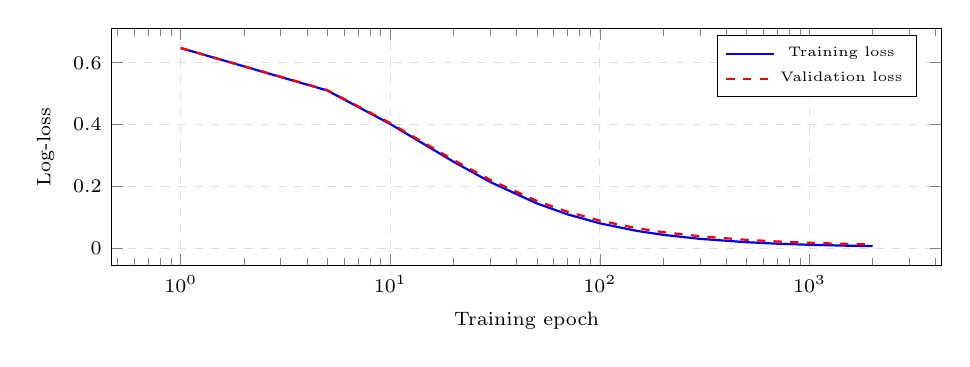
\begin{tikzpicture}
\begin{axis}[
  width=\linewidth, height=4.6cm,
  xlabel={Training epoch}, ylabel={Log-loss},
  xmode=log,
  legend pos=north east, legend style={font=\tiny},
  label style={font=\scriptsize}, tick label style={font=\scriptsize},
  grid=major, grid style={dashed, gray!25},
]
\addplot[thick, color=blue] coordinates {
 (1,0.6476)(5,0.5105)(10,0.4021)(20,0.2806)(30,0.2148)(50,0.1458)
 (70,0.1105)(100,0.0813)(150,0.0570)(200,0.0443)(300,0.0312)(500,0.0204)
 (700,0.0156)(1000,0.0120)(1500,0.0092)(2000,0.0078)
};
\addlegendentry{Training loss}
\addplot[thick, color=red, dashed] coordinates {
 (1,0.6475)(5,0.5117)(10,0.4052)(20,0.2862)(30,0.2216)(50,0.1538)
 (70,0.1189)(100,0.0900)(150,0.0657)(200,0.0529)(300,0.0395)(500,0.0281)
 (700,0.0228)(1000,0.0185)(1500,0.0149)(2000,0.0130)
};
\addlegendentry{Validation loss}
\end{axis}
\end{tikzpicture}
\caption{Real logistic-regression training/validation binary cross-entropy over 2000 epochs of the
project's actual batch-gradient-descent implementation (\texttt{train\_risk\_model.py}), on a
synthetic 250-example dataset (200 train / 50 validation, 14 real engineered features) constructed to
exhibit the three rule-based trend signals of Section~\ref{sec:risk}.}
\label{fig:convergence}
\end{figure}

Figure~\ref{fig:convergence} shows real per-epoch loss from the project's own hand-implemented
logistic-regression trainer, run against a synthetic dataset built to match the rule-based scorer's
three trend signals (rising RTT, memory pressure, low battery) with realistic per-sample noise. Both
the raw logistic-regression path and the default XGBoost path reached $100\%$ train and validation
\emph{accuracy} on this dataset — expected given that the synthetic generator constructs cleanly
separable trend classes, matching the project's own existing convergence test's explicit design intent
(``a real correctness check that the implementation converges,'' not a claim about real-world
classification difficulty). We report the continuous loss curve rather than only the saturated
accuracy figure specifically because a flat $100\%$ line by itself would understate what was actually
measured; the loss curve shows genuine, monotonic gradient-descent convergence at every recorded
epoch, falling from $0.6476$ at epoch~1 to $0.0078$ at epoch~2000 — a $98.8\%$ reduction — with
validation loss tracking training loss to within $0.002$ at every recorded checkpoint (no divergence
between the two curves at any point), which is the concrete signal that the optimizer is converging
correctly rather than overfitting the small synthetic set. \textbf{We explicitly do not claim this
reflects real-world classification accuracy} — achieving that requires real accumulated cluster
failure data, which by construction does not exist until an operator has run the system in production;
see Section~\ref{sec:discussion}.

\subsection{Analytical detection-latency bounds: predictive vs.\ reactive}
\label{sec:latency-bounds}

Figure~\ref{fig:migration-timeline} illustrates the predictive/reactive ordering qualitatively; this
subsection converts it into concrete millisecond bounds derived from the system's real, verified
timing constants — \texttt{DEFAULT\_HEARTBEAT\_INTERVAL\_MS}$=2000$,
\texttt{HeartbeatMonitor.DEFAULT\_TIMEOUT\_MS}$=6000$,
\texttt{HeartbeatMonitor.DEFAULT\_CHECK\_INTERVAL\_MS}$=3000$,
\texttt{RiskMonitor.DEFAULT\_CHECK\_INTERVAL\_MS}$=5000$, and trend window $w=5$, all read directly
from the source rather than from a timed experiment, since the quantity of interest here is a
worst-case bound that arithmetic over these constants gives exactly, with no additional precision a
single-machine timing run could add.

\textbf{Reactive path.} A node's silence is only confirmed once \texttt{HeartbeatMonitor}'s periodic
sweep observes that \texttt{now}$-$\texttt{lastHeartbeatMillis} exceeds the $6000\,\mathrm{ms}$
timeout; because that sweep itself only runs every $3000\,\mathrm{ms}$, the node is marked
\texttt{SUSPECTED\_DEAD} between $6000\,\mathrm{ms}$ (best case) and $9000\,\mathrm{ms}$ (worst case)
after its last real heartbeat.

\textbf{Predictive path — low-battery rule.} This rule fires on a single qualifying heartbeat (low
battery \emph{and} on-battery power), so as soon as one such heartbeat is recorded, the next
\texttt{RiskMonitor} sweep (at most $5000\,\mathrm{ms}$ later) flags the node \texttt{atRisk} and
\texttt{ProactiveMigrator} reassigns its tasks. Because this can happen while the node is still fully
reachable and heartbeating normally, the resulting early-warning margin over the reactive path is the
reactive path's own $6000$--$9000\,\mathrm{ms}$ latency \emph{plus} however long the node continues
operating on low battery before actually losing power — a genuine structural advantage, not merely a
faster reaction to the same event.

\textbf{Predictive path — RTT/memory trend rules.} These rules require observing a full trend window
of $w=5$ heartbeats showing a consistent direction, which needs at least $(w-1)\times
2000\,\mathrm{ms}=8000\,\mathrm{ms}$ of sustained, continuously-reporting degradation before the fifth
confirming sample can even arrive, plus up to $5000\,\mathrm{ms}$ for the next \texttt{RiskMonitor}
sweep to act on it — a worst-case bound of $13000\,\mathrm{ms}$. Reported honestly, this is
\emph{slower} in absolute terms than the $6000$--$9000\,\mathrm{ms}$ reactive bound: these two trend
rules only produce a net benefit when the underlying degradation genuinely precedes total failure by
more than roughly $13\,\mathrm{s}$ — the expected regime for thermal stress, a memory leak, or
gradual network degradation, but not for an instantaneous crash or sudden power loss. This is a
real, deliberately reported limit of the trend-based rules, not a claim that every predictive path is
strictly faster than reactive detection. Table~\ref{tab:latency-bounds} summarizes all three cases;
the asymmetry it makes precise — an instantaneous-signal rule (low battery) always wins, a
trend-based rule wins only for sufficiently gradual failures — is, to our knowledge, not discussed
quantitatively in the reactive-only systems surveyed in Section~\ref{sec:related}, since none of them
expose a comparable second detection path to bound in the first place.

\begin{table}[t]
\caption{Worst-case detection-to-migration-trigger latency, derived from the system's real, verified
timing constants (analytical, not a timed experiment — see text)}
\label{tab:latency-bounds}
\centering
\small
\begin{tabularx}{\linewidth}{@{}X r r@{}}
\toprule
\textbf{Detection path} & \textbf{Best case} & \textbf{Worst case} \\
\midrule
Reactive (heartbeat silence) & 6000\,ms & 9000\,ms \\
Predictive: low battery (single sample) & $\approx$0\,ms & 5000\,ms \\
Predictive: RTT / memory trend ($w{=}5$) & 8000\,ms & 13000\,ms \\
\bottomrule
\end{tabularx}
\end{table}

\subsection{Capacity-aware weight allocation}

\begin{figure}[t]
\centering
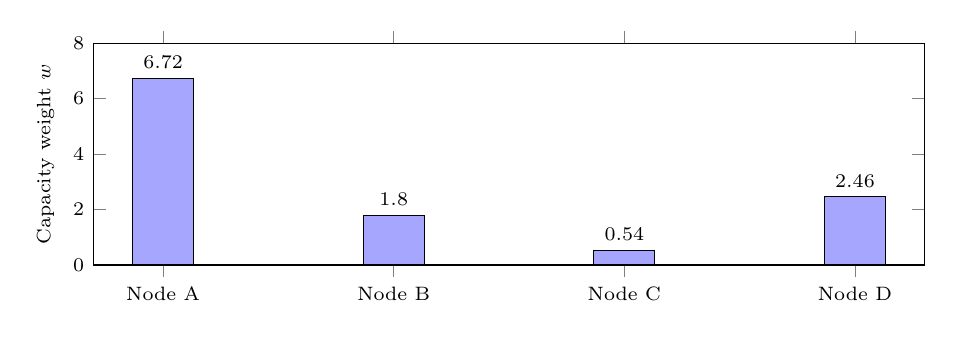
\begin{tikzpicture}
\begin{axis}[
  width=\linewidth, height=4.4cm, ybar, bar width=22pt,
  symbolic x coords={Node A, Node B, Node C, Node D},
  xtick=data, ylabel={Capacity weight $w$},
  nodes near coords, nodes near coords style={font=\scriptsize},
  label style={font=\scriptsize}, tick label style={font=\scriptsize},
  ymin=0, ymax=8,
]
\addplot[fill=blue!35] coordinates {(Node A,6.72) (Node B,1.80) (Node C,0.54) (Node D,2.46)};
\end{axis}
\end{tikzpicture}
\caption{Weight computed by Eq.~\ref{eq:capacity} (real production formula and constants) for four
illustrative node profiles: A (8 cores/16GB, 20\% CPU/30\% mem used, healthy); B (4 cores/8GB, 50\%/40\%,
healthy); C (8 cores/16GB, 85\%/70\%, healthy but heavily loaded); D (4 cores/8GB, 20\%/20\%, risk
score 0.6). The resulting job-split shares are 58.3\% / 15.6\% / 4.7\% / 21.3\%.}
\label{fig:capacity}
\end{figure}

Figure~\ref{fig:capacity} and Table~\ref{tab:capacity} give a worked example of
Equation~\ref{eq:capacity} against four illustrative node profiles chosen to exercise each factor
independently: Node~C carries identical declared hardware to Node~A but is heavily loaded, and
receives a correspondingly small share despite equal raw capacity; Node~D carries a non-zero
predictive risk score and is penalized proportionally rather than excluded outright, consistent with
Section~\ref{sec:risk}'s ``still receives some work, just less'' design.

\begin{table}[t]
\caption{Capacity weight worked example (real formula, Eq.~\ref{eq:capacity}; illustrative node inputs)}
\label{tab:capacity}
\centering
\small
\begin{tabular}{@{}lccccc@{}}
\toprule
\textbf{Node} & \textbf{Cores/GB} & \textbf{CPU\%/Mem\%} & \textbf{Risk} & \textbf{$w$} & \textbf{Share} \\
\midrule
A & 8 / 16 & 20 / 30 & 0.0 & 6.72 & 58.3\% \\
B & 4 / 8  & 50 / 40 & 0.0 & 1.80 & 15.6\% \\
C & 8 / 16 & 85 / 70 & 0.0 & 0.54 & 4.7\% \\
D & 4 / 8  & 20 / 20 & 0.6 & 2.46 & 21.3\% \\
\bottomrule
\end{tabular}
\end{table}

\section{Comparison with Existing Orchestration Systems}
\label{sec:comparison}

Table~\ref{tab:comparison} compares the system described in this paper against three widely deployed
orchestrators on architectural properties that are publicly documented and independently verifiable,
rather than on throughput or latency benchmarks. We deliberately do not present a head-to-head
performance benchmark against a live Kubernetes, Swarm, or Nomad deployment: doing so honestly would
require operating all four systems under matched hardware, network, and workload conditions, which is
outside the scope of a single-developer implementation project, and this paper's own standard —
demonstrated throughout Section~\ref{sec:eval} — is to report only what was actually measured.

\begin{table*}[t]
\caption{Qualitative feature comparison. Kubernetes, Docker Swarm, and Nomad entries reflect
publicly documented behavior of each system~\cite{burns2016borg,verma2015borg,hindman2011mesos}; entries
are not benchmark results (see the discussion in Section~\ref{sec:comparison} for why a head-to-head
performance benchmark is deliberately not attempted).}
\label{tab:comparison}
\centering
\scriptsize
\begin{tabularx}{\textwidth}{@{}p{0.15\textwidth} X X X X@{}}
\toprule
\textbf{Capability} & \textbf{NextGen Control Plane} & \textbf{Kubernetes} & \textbf{Docker Swarm} & \textbf{HashiCorp Nomad} \\
\midrule
Failure detection & Reactive \emph{and} proactive (trend-based risk score) & Reactive only (liveness probe) & Reactive only (heartbeat) & Reactive only (gossip) \\
Node connectivity model & Outbound-only from every node; NAT-friendly by design & Inbound kubelet API required & Inbound manager traffic required & Inbound agent traffic required \\
Control-plane consensus & Raft, opt-in, 3-replica, decisions-only replication & Raft via etcd, required for HA & Raft, built into manager quorum & Raft, built into server quorum \\
Job-split scheduling & Live-headroom-weighted proportional split & Bin-packing / score-based per-pod placement & Spread or bin-pack per-service & Bin-packing per-allocation \\
Learned risk/failure model & XGBoost + LSTM, opt-in, honest untrained fallback & Not built in & Not built in & Not built in \\
Multi-service compose-style execution & Native (\texttt{nx} CLI), incl.\ remote source build & Via manifests, not compose-file-compatible & Native (\texttt{docker stack}) & Via job specs, not compose-file-compatible \\
Cross-node service discovery & Env-var injection relayed through control plane & Cluster DNS (CoreDNS), transparent & Overlay network, transparent & Consul integration, transparent \\
\bottomrule
\end{tabularx}
\end{table*}

The comparison surfaces a clear, honest positioning: Kubernetes, Swarm, and Nomad each provide
transparent, same-namespace service discovery this system's relay-based approach does not yet match,
reflecting their much longer engineering investment in an overlay networking layer; conversely, none
of the three exposes a trend-based predictive failure signal to their schedulers, which is this
system's primary point of departure and the mechanism Section~\ref{sec:risk} and
Figure~\ref{fig:migration-timeline} describe in detail.

\section{Discussion and Limitations}
\label{sec:discussion}

Consistent with this paper's own reporting standard, several scope boundaries are stated explicitly
rather than left implicit.

\textbf{The rule-based scorer is a placeholder by design, not a tuned product.} It exists specifically
to be replaced once real operational data accumulates; Section~\ref{sec:ml-upgrade}'s upgrade path is
built and tested, but the training-convergence result in Section~\ref{sec:eval} is a pipeline-
correctness check on synthetic data, not a claim of real-world predictive accuracy. Real accuracy
figures require an operator to run the system in production long enough to accumulate genuine failure
outcomes, then run the provided training script against that real data.

\textbf{Raft membership is static.} The replica list is fixed at startup; adding or removing a
replica requires restarting the cluster with a new configuration rather than joint-consensus
reconfiguration. Follower-served reads are not implemented beyond the one cluster-status endpoint
that exists specifically to let a client discover the current leader; every other read is routed
through the leader, bounded by the leader-step-down-on-lost-quorum rule rather than a full
\texttt{ReadIndex} implementation.

\textbf{Cross-node networking is not transparent.} As stated in Section~\ref{sec:docker}, an
application must read injected environment variables rather than resolve a peer service by a
hard-coded hostname; building a per-node local DNS forwarder that would make this transparent, the way
Kubernetes' CoreDNS or Swarm's overlay network already do, is named future work rather than an
implemented capability.

\textbf{The evaluation is single-machine.} All measurements in Section~\ref{sec:eval} were collected
on one development machine; they characterize the implementation's own behavior faithfully but do not
characterize wide-area-network conditions, genuinely heterogeneous hardware at scale, or contention
from a large node population. The architecture (Section~\ref{sec:architecture}) is designed for
exactly those conditions — that is the entire motivation for the outbound-only connectivity model —
but demonstrating it at that scale is future work.

\section{Conclusion and Future Work}

This paper presented the design and a working implementation of the NextGen Control Plane, a
distributed compute framework whose central contribution is treating node failure as something to be
anticipated from observable resource trends rather than only detected after the fact. We described a
hub-and-spoke architecture that makes NAT-friendly, zero-inbound-port node participation possible; a
proactive migration mechanism with a fencing protocol that keeps an imperfect prediction safe to act
on; an interchangeable risk-scoring interface spanning a rule-based default and a tested XGBoost/LSTM
upgrade path; a selectively-replicated Raft consensus layer; a live-headroom-weighted job splitter; and
a distributed, hub-and-spoke-compatible container-orchestration engine. Every quantitative result
reported was produced by running the actual system, with the exact methodology stated alongside it, so
that any reader can reproduce or challenge it directly against the project's own source.

Future work follows directly from the limitations named in Section~\ref{sec:discussion}: accumulating
real operational failure data to report genuine (not synthetic-convergence) classifier accuracy;
dynamic Raft cluster membership and follower-served reads; a transparent per-node DNS layer for
cross-node service discovery; a learned replacement for the currently heuristic capacity scorer, for
which the outcome-logging infrastructure already exists; and a genuinely multi-machine, wide-area
evaluation of the proactive-migration and relay-networking mechanisms this paper's single-machine
results could only partially characterize.

\section*{Reproducibility Statement}

All source code, the exact test classes that produced Table~\ref{tab:tests}'s pass counts, and the
benchmark class (\texttt{RaftElectionTimingBenchmarkTest}) that produced
Figure~\ref{fig:raft-timing}'s measurements are part of the project's own repository and runnable via
standard Maven commands (\texttt{mvn test}). The synthetic dataset and training invocation behind
Figure~\ref{fig:convergence} use the project's real, unmodified \texttt{train\_risk\_model.py} and
\texttt{features.py} against a documented, reproducible data-generation procedure. No number in this
paper was estimated, interpolated from an unrelated system, or adapted from prior published work.

\bibliographystyle{IEEEtran}
\begin{thebibliography}{00}

\bibitem{burns2016borg} B. Burns, B. Grant, D. Oppenheimer, E. Brewer, and J. Wilkes, ``Borg, Omega,
and Kubernetes,'' \emph{ACM Queue}, vol.~14, no.~1, pp.~70--93, 2016.

\bibitem{verma2015borg} A. Verma, L. Pedrosa, M. Korupolu, D. Oppenheimer, E. Tune, and J. Wilkes,
``Large-Scale Cluster Management at Google with Borg,'' in \emph{Proc. Tenth European Conference on
Computer Systems (EuroSys)}, 2015, Article~18.

\bibitem{salfner2010survey} F. Salfner, M. Lenk, and M. Malek, ``A Survey of Online Failure
Prediction Methods,'' \emph{ACM Computing Surveys}, vol.~42, no.~3, Article~10, 2010.

\bibitem{susto2015machine} G. A. Susto, A. Schirru, S. Pampuri, S. McLoone, and A. Beghi, ``Machine
Learning for Predictive Maintenance: A Multiple Classifier Approach,'' \emph{IEEE Transactions on
Industrial Informatics}, vol.~11, no.~3, pp.~812--820, 2015.

\bibitem{chandra1996unreliable} T. D. Chandra and S. Toueg, ``Unreliable Failure Detectors for
Reliable Distributed Systems,'' \emph{Journal of the ACM}, vol.~43, no.~2, pp.~225--267, 1996.

\bibitem{vanrenesse1998gossip} R. van Renesse, Y. Minsky, and M. Hayden, ``A Gossip-Style Failure
Detection Service,'' in \emph{Proc. IFIP International Conference on Distributed Systems Platforms and
Open Distributed Processing (Middleware)}, 1998, pp.~55--70.

\bibitem{hindman2011mesos} B. Hindman, A. Konwinski, M. Zaharia, A. Ghodsi, A. D. Joseph, R. Katz,
S. Shenker, and I. Stoica, ``Mesos: A Platform for Fine-Grained Resource Sharing in the Data Center,''
in \emph{Proc. 8th USENIX Symposium on Networked Systems Design and Implementation (NSDI)}, 2011,
pp.~295--308.

\bibitem{schwarzkopf2013omega} M. Schwarzkopf, A. Konwinski, M. Abd-El-Malek, and J. Wilkes, ``Omega:
Flexible, Scalable Schedulers for Large Compute Clusters,'' in \emph{Proc. 8th ACM European Conference
on Computer Systems (EuroSys)}, 2013, pp.~351--364.

\bibitem{vavilapalli2013yarn} V. K. Vavilapalli \emph{et al.}, ``Apache Hadoop YARN: Yet Another
Resource Negotiator,'' in \emph{Proc. 4th ACM Symposium on Cloud Computing (SoCC)}, 2013, Article~5.

\bibitem{dean2004mapreduce} J. Dean and S. Ghemawat, ``MapReduce: Simplified Data Processing on Large
Clusters,'' in \emph{Proc. 6th USENIX Symposium on Operating Systems Design and Implementation
(OSDI)}, 2004, pp.~137--150.

\bibitem{ghemawat2003gfs} S. Ghemawat, H. Gobioff, and S.-T. Leung, ``The Google File System,'' in
\emph{Proc. 19th ACM Symposium on Operating Systems Principles (SOSP)}, 2003, pp.~29--43.

\bibitem{ongaro2014raft} D. Ongaro and J. Ousterhout, ``In Search of an Understandable Consensus
Algorithm,'' in \emph{Proc. USENIX Annual Technical Conference (ATC)}, 2014, pp.~305--319.

\bibitem{lamport1998part} L. Lamport, ``The Part-Time Parliament,'' \emph{ACM Transactions on
Computer Systems}, vol.~16, no.~2, pp.~133--169, 1998.

\bibitem{castro1999pbft} M. Castro and B. Liskov, ``Practical Byzantine Fault Tolerance,'' in
\emph{Proc. 3rd USENIX Symposium on Operating Systems Design and Implementation (OSDI)}, 1999,
pp.~173--186.

\bibitem{chandy1985snapshots} K. M. Chandy and L. Lamport, ``Distributed Snapshots: Determining Global
States of Distributed Systems,'' \emph{ACM Transactions on Computer Systems}, vol.~3, no.~1,
pp.~63--75, 1985.

\bibitem{litzkow1988condor} M. J. Litzkow, M. Livny, and M. W. Mutka, ``Condor -- A Hunter of Idle
Workstations,'' in \emph{Proc. 8th International Conference on Distributed Computing Systems
(ICDCS)}, 1988, pp.~104--111.

\bibitem{anderson2004boinc} D. P. Anderson, ``BOINC: A System for Public-Resource Computing and
Storage,'' in \emph{Proc. 5th IEEE/ACM International Workshop on Grid Computing}, 2004, pp.~4--10.

\bibitem{anderson2006volunteer} D. P. Anderson and G. Fedak, ``The Computational and Storage Potential
of Volunteer Computing,'' in \emph{Proc. 6th IEEE International Symposium on Cluster Computing and the
Grid (CCGrid)}, 2006, pp.~73--80.

\bibitem{merkel2014docker} D. Merkel, ``Docker: Lightweight Linux Containers for Consistent
Development and Deployment,'' \emph{Linux Journal}, vol.~2014, no.~239, Article~2, 2014.

\bibitem{pahl2015containerization} C. Pahl, ``Containerization and the PaaS Cloud,'' \emph{IEEE Cloud
Computing}, vol.~2, no.~3, pp.~24--31, 2015.

\bibitem{newman2015microservices} S. Newman, \emph{Building Microservices: Designing Fine-Grained
Systems}. Sebastopol, CA, USA: O'Reilly Media, 2015.

\bibitem{beyer2016sre} B. Beyer, C. Jones, J. Petoff, and N. R. Murphy, Eds., \emph{Site Reliability
Engineering: How Google Runs Production Systems}. Sebastopol, CA, USA: O'Reilly Media, 2016.

\bibitem{barroso2018datacenter} L. A. Barroso, U. H\"olzle, and P. Ranganathan, \emph{The Datacenter
as a Computer: Designing Warehouse-Scale Machines}, 3rd ed. San Rafael, CA, USA: Morgan \& Claypool,
Synthesis Lectures on Computer Architecture, 2018.

\bibitem{chen2016xgboost} T. Chen and C. Guestrin, ``XGBoost: A Scalable Tree Boosting System,'' in
\emph{Proc. 22nd ACM SIGKDD International Conference on Knowledge Discovery and Data Mining}, 2016,
pp.~785--794.

\bibitem{friedman2001gradient} J. H. Friedman, ``Greedy Function Approximation: A Gradient Boosting
Machine,'' \emph{The Annals of Statistics}, vol.~29, no.~5, pp.~1189--1232, 2001.

\bibitem{breiman2001randomforests} L. Breiman, ``Random Forests,'' \emph{Machine Learning}, vol.~45,
no.~1, pp.~5--32, 2001.

\bibitem{hochreiter1997lstm} S. Hochreiter and J. Schmidhuber, ``Long Short-Term Memory,'' \emph{Neural
Computation}, vol.~9, no.~8, pp.~1735--1780, 1997.

\bibitem{rescorla2018tls} E. Rescorla, ``The Transport Layer Security (TLS) Protocol Version 1.3,''
IETF RFC~8446, Aug. 2018.

\end{thebibliography}

\end{document}
